General Regression: find $\hat{y} = f(x) \leftrightarrow \underset{\hat{y}(x)}{min} ||y - \hat{y}(x)||_2^2$.

$f^*(x)$ that minimizes L is $\mathbb{E}[X|\boldsymbol{X=x}]$ called \textbf{Bayes Optimal Predictor}. In practice unattainable.

Linear Regression: Weights are applied linearly:

$f(x) = \omega x$ or nonlinear \textbf{base fct}: $f(x) = \omega\phi(x)$

Multidim.: $L = \underset{\omega}{min}||\boldsymbol{Y-X\omega||}^2$, 

$Y \in \mathbb{R}^n, x \in \mathbb{R}^{nxd},\omega \in \mathbb{R}^d$

\subsection{Closed Solution}

If $X^TX $ is invertible $ (X^TX\text{ has full rank} \Leftrightarrow rank(X) = min(d,n)) \Rightarrow$ closed solution: $\omega = \boldsymbol{(X^TX)^{-1}X^TY}$

$\nabla L$ is $\mathbb{O}(nd)$, closed solution is $\mathbb{O}(nd^2)$.

Alternatively geom. proj.: $(\boldsymbol{y - X\hat{\omega}})^TX\omega = 0$
\subsection{Optimization}

    If not solvable in closed form or expensive to invert $X^TX\rightarrow$ Gradient Descent:
    
    $\omega_{t+1} \leftarrow \omega_t - \eta \nabla L(\boldsymbol{\omega_t})$, $\eta$ is the learning rate.
    
    Convergence guaranteed for $\eta \geq \frac{2}{\lambda_{max}}$, where $\lambda_{max}$ is the max EV of $X^TX$. 
    
    $X^TX$ diagonal $\Rightarrow$ contour lines ($L$ const) are ellipses
    
    
\subsection{Nonlinear Regression}

\textbf{Note: } When working with NNs both the weights and the nonlinear functions are chosen.

For closed solution same applies rank$\phi(x) \overset{!}{=} min(n,p)$
\subsection{Regularization}

Among all unbiased solutions $(X^TX)^{-1}X^TY$ is the solution that has the smallest variance $\Rightarrow$ minimizes gen. Error

One can set the $\omega$ of higher order features manually to zero ($\leftrightarrow$ choose a less complex model) or

\textbf{Ridge Regression} $\underset{\omega}{min}||Y-X\omega||^2 + \lambda||\omega||^2$

Always allows for closed solution and lets LS converge faster (EVs of Hessian $X^TX$ change)

Equivalent to performing Bayesianism approach with $p(\omega) = \mathcal{N}(\omega|0,\boldsymbol{\Lambda}^{-1})$ or linearly $p(\omega) = \mathcal{N}(\omega|0,1)$

\textbf{Lasso Regression} $\underset{\omega}{min}||Y-X\omega||^2 + \lambda|\omega|$ 

Convex loss  but no closed form solution (not differentiable)

Bayes. w/ Laplacian prior:  $p(\omega_i) = \frac{\lambda}{4\sigma^2}exp(-|\omega_i|\frac{\lambda}{w\sigma^2})$

$\omega_{\text{high}} \rightarrow 0 \Rightarrow$ sparse, $\lambda_{opt}$ through CV.

% \begin{center}
%     \resizebox{0.6\linewidth}{!}{
%     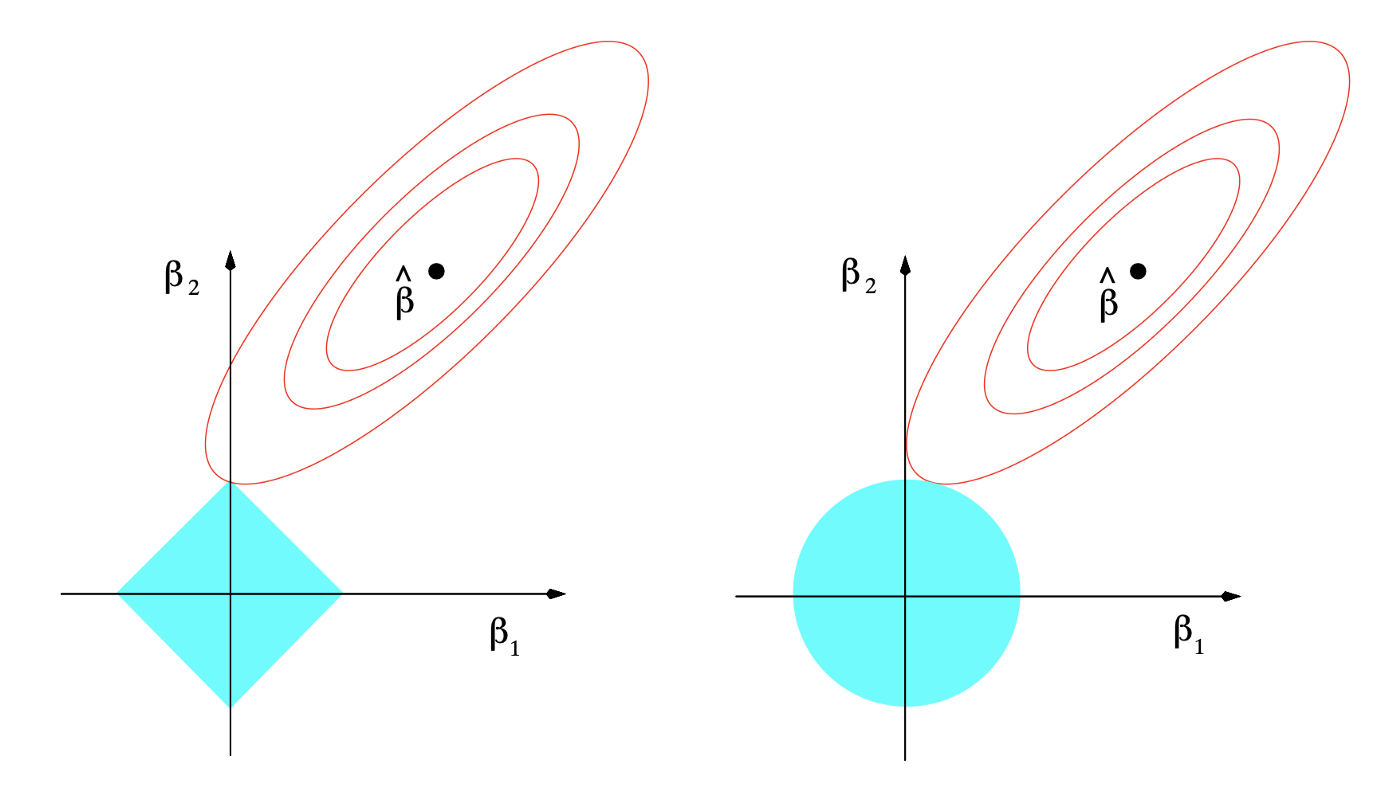
\includegraphics{images/lasso_vs_ridge.png}
%     }
% \end{center}
% Left: Lasso, Right: Ridge



